\chapter{Additional analysis constraints \label{chap:advection}}
\vspace*{-1cm}
\lettrine[lines=2, loversize=-0.1, lraise=0.1]{D}{iva} software offers the possibility of considering a velocity field that will influence the results of the analysis through advection. 

\minitoc


\section{Introduction}
%---------------------------------

Activating an advection constraint on the tracers is done by adding a term to the norm of the field $\varphi$ \eqref{divaformula2}, leading to

\begin{equation}
\tilde{J}= J(\varphi) + \frac{\theta}{U^2 L^2} \int_{\tilde{D}}\left[
\vect{u} \cdot \tilde{\nabla} \varphi
- \frac{\mathcal{A}}{L} \, \tilde{\nabla}\! \cdot\! \tilde{\nabla}\varphi
\right]^2 \ddiff \tilde{D}
\end{equation}

where $U$ and $L$ are characteristic velocity and length scales, respectively. The parameter $\theta$ allows one to adapt the weight of the additional second term, in which we recognize a stationary advection-diffusion equation. The physical meaning of the term $\vect{u} \cdot \tilde{\nabla} \varphi$ is simple: when the velocity is nearly parallel to the gradient, the product has a large value and is thus penalized. Then for a strong constraint ($\theta\gg 1$) we enforce the analysis to align with velocity.

In general we can assume $\mathcal{A} \le U L$, in other words, we work at relatively high \textit{Reynolds numbers} \footnote{The Reynolds number measures the ratio of the inertial effects over the viscosity effects}. Otherwise for dominant diffusion, the term just adds another isotropic filtering effect, already included in the regularization term (Eq. \ref{divaformula2}). Hence the additional term is really interesting only for situations dominated by advection, with $\mathcal{A} \le U L$. In this case, the scaling is such that for $\theta\approx 1$, the advection constraint has a similar importance with respect to the regularization term.

The velocity scale $U$ is calculated from the provided $\vect{u}=(u,v)$ field. 

Note that when using the advection constraint, the correlation length provided by {\tt divafit} should be decreased since the advection 
constraint implicitly increases correlation length along currents.


\section{Illustrations}
%------------------------

\subsection{Advection alone}
%------------------------------

Fig. \ref{fig:solidrot} shows an example of a single data point in\, $(0.7,60)$ with unit value in a solid 
rotation (centred in $(0,60)$). In the absence of diffusion, up and downwind are identical (covariance 
counts).

\begin{figure}[H]
\parbox{.6\textwidth}{
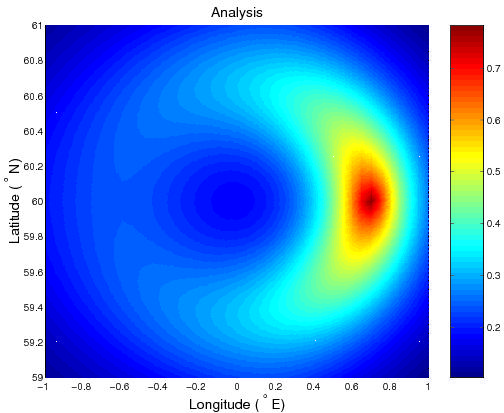
\includegraphics[width=.55\textwidth]{solidrot}
}\parbox{.4\textwidth}{
\caption{Single data point with unit value in a solid 
rotation. \label{fig:solidrot}}
}
\end{figure}


Without advection (Fig. \ref{fig:norot}), the across velocity scale remains and isotropy is 
recovered (except for boundary effect on the right side).

\begin{figure}[H]
\parbox{.6\textwidth}{
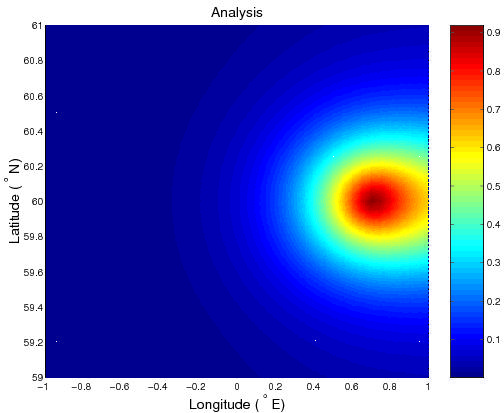
\includegraphics[width=.55\textwidth]{norot}
}\parbox{.4\textwidth}{
\caption{Same as Fig. \ref{fig:solidrot}, but without advection. \label{fig:norot}}
}
\end{figure}



To decrease the across frontal scale, we must decrease $L$ but add advection 
to keep along-current scale larger (Fig. \ref{fig:solidrotsmall}).

\begin{figure}[H]
\parbox{.6\textwidth}{
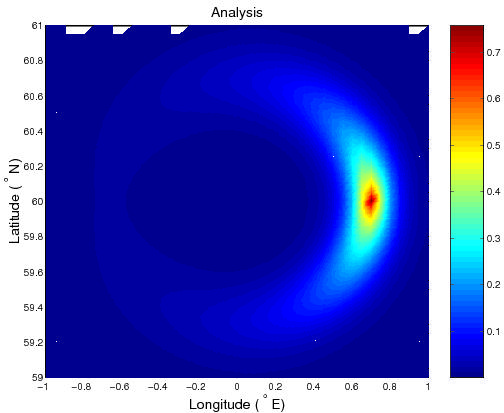
\includegraphics[width=.55\textwidth]{solidrotsmall}
}\parbox{.4\textwidth}{
\caption{Same as Fig. \ref{fig:solidrot}, but with smaller length scale. \label{fig:solidrotsmall}}
}
\end{figure}


Adding advection without decreasing $L$ increases correlation length 
along front and keeps across front correlation length.

\subsection{Advection and diffusion}
%--------------------------------------

Adding diffusion makes possible the distinction between up and downwind 
direction (Fig. \ref{fig:solidrotp}): in this case, higher values are found upwind of the data 
location: this is natural, because the data is observed and \diva\, tries to 
infer the field that explains the sample. This requests higher values 
upwind (because downwind values decrease).

Because of the square in the formulation, to change the flow direction 
you can simply change the sign of the diffusion coefficient or change 
the sign of the velocity components (Fig. \ref{fig:solidrotm}).

\begin{figure}[htpb]
\parbox{.6\textwidth}{
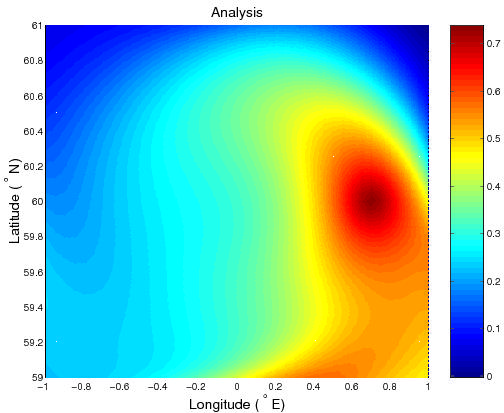
\includegraphics[width=.55\textwidth]{solidrotp}
}\parbox{.4\textwidth}{
\caption{Single data point with anti-clockwise rotation and with diffusion. \label{fig:solidrotp}}
}
\end{figure}

\begin{figure}[htpb]
\centering
\parbox{.6\textwidth}{
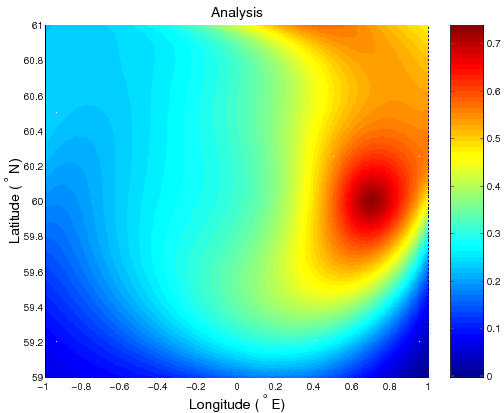
\includegraphics[width=.55\textwidth]{solidrotm}
}\parbox{.4\textwidth}{
\caption{Single data point with clockwise rotation and with diffusion. \label{fig:solidrotm}}
}
\end{figure}





\section{Generalization}
%--------------------------

Zero diffusion simply leads to correlations that are increased in the 
direction of the vector $\vect{u}$ (or decreased in the perpendicular 
direction if the global $L$ is increased simultaneously). 

The vector $\vect{u}$ does not need to be a velocity in this case, but can be any 
vector indicating the direction in which correlation is to be increased.
Hence it could be for example, topography gradients rotated by $90$ degrees 
or density gradients rotated by 90 degrees if we respectively assume across depth-contour movements are more 
difficult (and hence data correlation decreased) or across frontal movements more difficult (and hence correlation length 
across fronts decreased).

The advection constraint therefore allows any known anisotropy in the correlations to be included into the analysis. We notice that the vector field does not need to be divergence free.



% \section{Error field}

% provided by diva, but interpretation different as the normal case
% need to add more details on this
